\documentclass[11pt,letterpaper,boxed, noheader]{pset}

\usepackage[margin=0.75in]{geometry, caption}
\usepackage{ulem}

\begin{document}

    \problemlist{PHYS051 HW15}
    \begin{center}
        T1.37; T1.43
    \end{center}
    
    \begin{problem} [T1.37]
        Determine the probability that a photon is detected at the first minimum of a six-slit grating if the bottom two slits were closed. Assume that the magnitude of the probability amplitude due to each slit is $r$. \textit{Suggestion:} Start by showing how the complex probability amplitudes from each slit add up to zero at the first minimum.
    \end{problem}
    \newpage
    
    \begin{problem} [T1.43]
        Use the principle of least time to derive Snell's law, namely, $n_1 \text{sin} \theta_1 = n_2 \text{sin} \theta_2$ for light being refracted as it travels from a medium with index of refraction $n_1$ into a medium with index of refraction $n_2$. \textit{Suggestion:} Follow a procedure similar to the one given in Example 1.11. Locate the source S in medium 1 and the point P in medium 2.
    \end{problem}
    \newpage
    
    \begin{problem} [Example 1.11]
        Use Fermat's principle of least time to derive the law of reflection, namely, that the angle of incidence is equal to the angle of reflection. 
    \end{problem}
    
    \begin{figure} [ht]
    \begin{solution}
        For the most generality, assume that the source S and the detector P are at different elevations above the mirror, as indicated in Fig. 1.41. The time for light to travel from S to P is given by 
        \[ t = \frac{1}{c} (\sqrt{a^2 + x^2} + \sqrt{(D-x)^2 + b^2}) \]
        Minimizing the time by varying $x$, we find that
        \[ \frac{dt}{dx} = \frac{1}{c} (\frac{x}{\sqrt{a^2+x^2}} - \frac{D-x}{\sqrt{(D-x)^2 + b^2}}) = 0 \]
        or
        \[ \frac{x}{\sqrt{a^2+x^2}} = \frac{D-x}{\sqrt{(D-x)^2 + b^2}}\]
        
        \begin{center}
            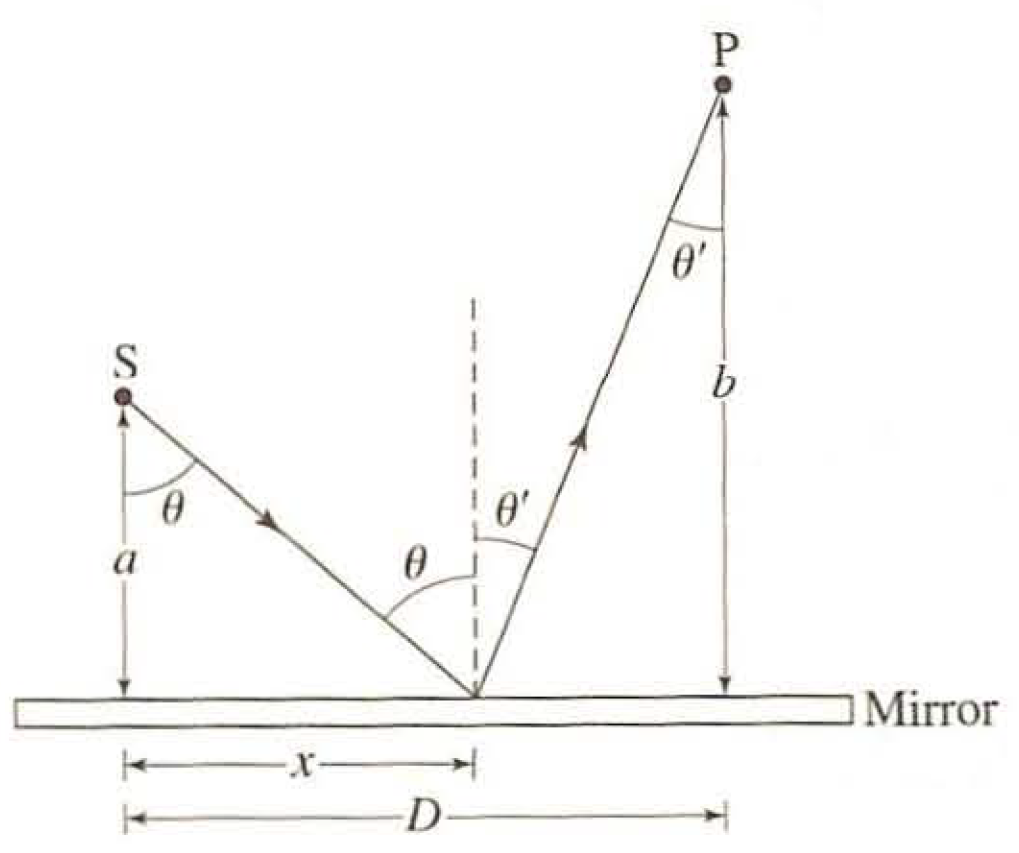
\includegraphics[width=150px]{HW15Images/Ex1-11.png}
            \captionsetup{labelformat=empty} \caption*{\textit{A general path between source S and detector P in the reflection of light from a mirror.}}
        \end{center}
        
        \bigskip
        In terms of the angles shown in the figure above, this can be simply written as 
        \[ \text{sin}\theta = \text{sin}\theta' \]
        or $\theta = \theta'$, namely, the angle of incidence equals the angle of reflection. Problem 1.43 shows how Fermat's principle can be used to derive Snell's law $(n_1 \text{sin}\theta_1 = n_2 \text{sin}\theta_2)$ for light refracted from a medium with index of refraction $n_1$ into a medium with index of refraction $n_2$.
    \end{solution}
    \end{figure}
\end{document}